\documentclass{article}

\usepackage[margin=1in]{geometry}
\usepackage{amssymb}
\usepackage{amsmath}
\usepackage{indentfirst}
\usepackage{algorithm}
\usepackage[noend]{algpseudocode}
\usepackage{underscore}
\usepackage{placeins}
\usepackage{graphicx}
\usepackage{multirow}
\usepackage{longtable}

\begin{document}

\title{CSCI 6100 \protect\\ Research Project Report \protect\\ Largest Rectangle of 1's in a Matrix}
\author{Cruz Jean}
\maketitle

\FloatBarrier
\begin{figure}[!ht]
\centering
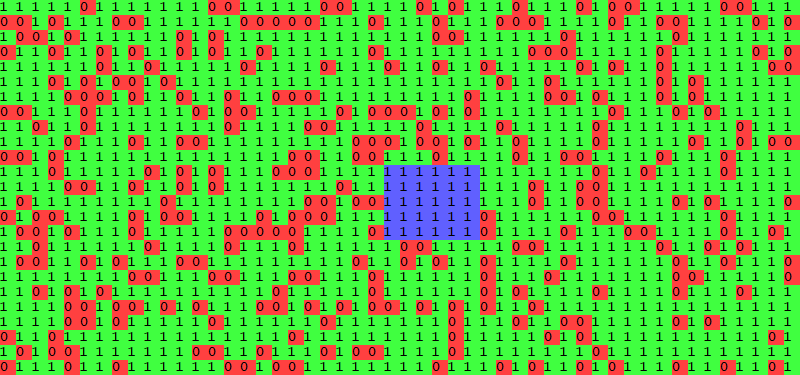
\includegraphics[width=140mm]{titleImage.png}
\end{figure}
\FloatBarrier

\pagebreak
\section{Introduction}

In this problem, we are given a matrix that contains only zeros and ones.
We must find the largest rectangular subregion that contains only ones.

We will explore two algorithms to accomplish this: one using a branch and bound approach and one using a dynamic programming approach.
Additionally, we will perform the theoretical analysis for both algorithms and verify the results with experimental data taken from \texttt{C++} implementations.


\section{Background}

This problem is a specialized form of several more-general problems.
One such problem is finding the largest convex region of 1's in a matrix, where we would need to define convexity for a discrete (raster) coordinate space (e.g. any region consisting of one or more rectangles that all contain a common point).
The most general form is the problem of finding the largest contiguous (potentially concave) region of 1's in a matrix.
These are clearly more general due to not requiring the region be rectangular, but in allowing this they become significantly more difficult to solve.

This problem lies in the large category of searching problems, as we are searching for a particular region of the matrix with a certain set of properties.
However, this also lies in the category of optimization problems, as there are many possible rectangles of 1's in any given matrix but we want to find the largest of them (without even knowing how big the solution might be).

These are arguably two of the most important types of problems to solve from an efficiency standpoint.
For instance, a program that solves a Rubik's cube would fall in this same sort of category:
it's searching for a sequence of moves to make that will solve the configuration,
and it's simultaneously trying to find the fastest way to do so.
We (users) typically think of a Rubik's cube solver as being very fast, to the point that any smartphone can do it in a matter of seconds.
However in the worst case its time complexity can still be exponential in the number of moves that must be made.
This is actually rather common for searching problems, and is the reason why having powerful and efficient algorithms to accelerate this process is so important.
Without good search algorithms the required execution time would quickly become intractable and the algorithm effectively useless.

However, the situation regarding this algorithm in particular (i.e. the largest rectangle of 1's in a matrix) is not nearly so grim. Our problem is much simpler than solving a Rubik's cube due to having a finite search space and simple rules that can be used to eliminate many otherwise-redundant failed states (e.g. any region that's not a rectangle or that contains a zero).

In fact our problem is simple enough that it begins to have parallels with some (extremely) simple algorithms such as finding the largest value in an array.
This can be seen by taking a much more restricted look at the problem: finding the largest \textit{square} of 1's in a matrix.
In this case the most efficient solution effectively amounts to sweeping a wall of local maxima through the entire matrix and  taking the final highest of the highest values (think dynamic programming).

Another similar problem is the problem of determining the optimal way to cut an arbitrary raster region into a union of disjoint rectangles (i.e. no overlap).
For instance, one such algorithm to do so (which is perhaps sub-optimal) would be to use this algorithm to find the largest rectangle in the region, add it as a rectangle in the union, remove the rectangle from the total region, and repeat until nothing remains.

\section{Problem Description}

We're given an $n \times m$ matrix of ones and zeros.
We must find the largest rectangular region in the matrix that consists of only 1's, including both its location and dimensions.
Such a region may not be unique.
In the case of non-unique optimal solutions, any will suffice.

\pagebreak
\section{Branch and Bound Approach}

\textbf{Problem:}
We're given an $n \times m$ matrix of ones and zeros.
We must find the largest rectangular region in the matrix that consists of only 1's, including both its location and dimensions.
Such a region may not be unique.
In the case of non-unique optimal solutions, any will suffice.

\textbf{Inputs:}
The $n \times m$ matrix.

\textbf{Outputs:}
The largest rectangular region of 1's that was found during the search, defined as a pair of $(row, col)$ represents the top left corner of the rectangle and $(height, width)$ represent its dimensions.

\FloatBarrier
\begin{algorithm}
\caption{Branch and Bound Algorithm}
\begin{algorithmic}[1]
\Function{BranchAndBound}{$matrix$}
	\State $solution \gets ((0, 0), (0, 0))$
	\State $best\_solution \gets ((0, 0), (0, 0))$
	\State $best\_size \gets 0$
	
	\For{$solution[0][0] = 0 \texttt{ ; } solution[0][0] < rows(matrix) \texttt{ ; } \texttt{++}solution[0][0]$}
		\For{$solution[0][1] = 0 \texttt{ ; } solution[0][1] < cols(matrix) \texttt{ ; } \texttt{++}solution[0][1]$}
			\State $solution[1][0] \gets 1$
			\While {\texttt{True}}
				\If {$solution[0][0] + solution[1][0]-1 < len(matrix)$} \texttt{break} \EndIf
				\If {$matrix[solution[0][0]+solution[1][0]-1][solution[0][1]]$} \texttt{break} \EndIf

				\For{$solution[1][1] = 1 \texttt{ ; } \Call{IsValid}{$matrix, solution$} \texttt{ ; } \texttt{++}solution[1][1]$}
					\State $size \gets solution[1][0] \times solution[1][1]$
					\If {$size > best\_size$}
						\State $best\_solution \gets solution$
						\State $best\_size \gets size$
					\EndIf
				\EndFor
				\State $solution[1][0] \gets solution[1][0] + 1$
			\EndWhile
		\EndFor
	\EndFor

	\State \Return $best\_solution$
\EndFunction
\end{algorithmic}
\end{algorithm}
\FloatBarrier

\FloatBarrier
\begin{algorithm}
\caption{Check if Solution is Valid}
\begin{algorithmic}[1]
\Function{IsValid}{$matrix, solution$}
	\If {$solution[0][0]+solution[1][0] > rows(matrix)$} \Return \texttt{False} \EndIf
	\If {$solution[0][1]+solution[1][1] > cols(matrix)$} \Return \texttt{False} \EndIf

	\For {$i = 0 \texttt{ ; } i < solution[1][0] \texttt{ ; } \texttt{++}i$}
		\For {$j = 0 \texttt{ ; } j < solution[1][1] \texttt{ ; } \texttt{++}j$}
			\If {$\texttt{not } matrix[solution[0][0] + i][solution[0][1] + j]$} \Return \texttt{False} \EndIf
		\EndFor
	\EndFor

	\State \Return \texttt{True}
\EndFunction
\end{algorithmic}
\end{algorithm}
\FloatBarrier

\subsection {Theoretical Best Case Analysis}

In this algorithm, regardless of the contents of the matrix, every single position must be visited (to see if it's a zero or a one).
The more expensive logic is done in the case that ones are encountered.
Thus, the best case is created by having the entire marix be filled with zeros, which causes the third loop to exit immediately.
And so we can express our worst case complexity quite simply:

\begin{align}
B(n) &= \sum_{i=1}^n {\sum_{j=1}^m {1}} = nm \in \mathcal{O}(nm)
\end{align}

And so we have that the best case complexity is linear in the number of items in the matrix.
Given that we have no other information about the matrix, this is optimal, as we must at the very least examine every position of the matrix to determine any answer.

\subsection {Theoretical Worst Case Analysis}

Similarly, the worst case is created by having a matrix entirely composed of ones.
This forces all four loops to run in their entirety, examining every rectangular subregion of the matrix.

\begin{align}
W(n) &= \sum_{i=1}^n {\sum_{j=1}^m {\sum_{x=1}^i{\sum_{y=1}^j{xy}}}} \\
&= \sum_{i=1}^n {\sum_{j=1}^m {\sum_{x=1}^i{x \sum_{y=1}^j{y}}}} \\
&= \sum_{i=1}^n {\sum_{j=1}^m {\sum_{x=1}^i{x \frac{j(j+1)}{2}}}} \\
&= \sum_{i=1}^n {\sum_{j=1}^m {\frac{j(j+1)}{2}\sum_{x=1}^i{x}}} \\
&= \sum_{i=1}^n {\sum_{j=1}^m {\frac{j(j+1)}{2}\frac{i(i+1)}{2}}} \\
&= \sum_{i=1}^n {\frac{i(i+1)}{2}\sum_{j=1}^m {\frac{j(j+1)}{2}}} \\
&= \left(\sum_{i=1}^n {\frac{i(i+1)}{2}}\right)\left(\sum_{j=1}^m {\frac{j(j+1)}{2}}\right) \\
&= \frac{1}{4}\left(\sum_{i=1}^n {i^2+i}\right)\left(\sum_{j=1}^m {j^2+j}\right) \\
&= \frac{1}{4}\left( \frac{n(n+1)(2n+1)}{6} + \frac{n(n+1)}{2} \right)\left( \frac{m(m+1)(2m+1)}{6} + \frac{m(m+1)}{2} \right) \\
&= \frac{1}{144}\left( n(n+1)(2n+1) + 3n(n+1) \right)\left( m(m+1)(2m+1) + 3m(m+1) \right) \\
&= \frac{1}{144}\left( n(n+1)(2n+4) \right)\left( m(m+1)(2m+4) \right) \\
&= \frac{1}{36} n(n+1)(n+2)m(m+1)(m+2) \\
&\in \mathcal{O}(n^3m^3)
\end{align}

Thus we have that this algorithm is quite inefficient in the worst case, growing with the cube of the number of items in the matrix.
The critical variable that determines the efficiency of this algorithm is the distribution of zeros and ones in the matrix.

\pagebreak
\section{Dynamic Programming Approach}

\textbf{Problem:}
We're given an $n \times m$ matrix of ones and zeros.
We must find the largest rectangular region in the matrix that consists of only 1's, including both its location and dimensions.
Such a region may not be unique.
In the case of non-unique optimal solutions, any will suffice.

\textbf{Inputs:}
The $n \times m$ matrix.

\textbf{Outputs:}
The largest rectangular region of 1's that was found during the search, defined as a pair of $(row, col)$ represents the top left corner of the rectangle and $(height, width)$ represent its dimensions.

\FloatBarrier
\begin{algorithm}
\caption{Dynamic Programming Algorithm}
\begin{algorithmic}[1]
\Function{Dynamic}{$matrix$}
	\State $histogram[cols(matrix)] \gets [0, ... ]$
	\State $best \gets ((0,0),(0,0))$
	\State $best\_area \gets 0$

	\For {$i = 0 \texttt{ ; } i < rows(matrix) \texttt{ ; } \texttt{++}i$}
		\For {$j = 0 \texttt{ ; } j < cols(matrix) \texttt{ ; } \texttt{++}j$}
			\If {$matrix[i][j]$}
				\State $histogram[j] \gets histogram[j] + 1$
			\Else
				\State $histogram[j] \gets 0$
			\EndIf

			\State $res \gets \Call{MaxHistogramRect}{histogram}$
			\State $area \gets res[1] \times res[2]$
			
			\If {$area > best\_area$}
				\State $best\_area \gets area$
				\State $best \gets ((i-res[2]+1,res[0]),(res[2],res[1]))$
			\EndIf
		\EndFor
	\EndFor

	\State \Return $best$
\EndFunction
\end{algorithmic}
\end{algorithm}
\FloatBarrier

\FloatBarrier
\begin{algorithm}
\caption{Find Largest Rectangle in a Histogram}
\begin{algorithmic}[1]
\Function{MaxHistogramRect}{$histogram$}
	\State $stack \gets []$
	\State $i, best\_area \gets 0, 0$
	\State $best\_left, best\_width, best\_height \gets 0, 0, 0$

	\State $pop\_one \gets \texttt{lambda}$ () \{
		\State \hspace{\algorithmicindent} $prev \gets pop(stack)$
		\State \hspace{\algorithmicindent} $area \gets histogram[top] \times (empty(stack) \texttt{ ? } i \texttt{ : } i - 1 - top(stack))$
		\State \hspace{\algorithmicindent} {\textbf{if} $area > best\_area$ \textbf{then}}
			\State \hspace{\algorithmicindent} \hspace{\algorithmicindent} $best\_area \gets area$
			\State \hspace{\algorithmicindent} \hspace{\algorithmicindent} $best\_left \gets empty(stack) \texttt{ ? } 0 \texttt{ : } 1 + top(stack)$
			\State \hspace{\algorithmicindent} \hspace{\algorithmicindent} $best\_width \gets empty(stack) \texttt{ ? } i \texttt{ : } i - 1 - top(stack)$
			\State \hspace{\algorithmicindent} \hspace{\algorithmicindent} $best\_height \gets histogram[prev]$
	\State \}

	\While {$i < len(histogram)$}
		\If {$empty(stack) \texttt{ or } histogram[top(stack)] \leq histogram[i]$}
			\State $push(stack, i)$
			\State $i \gets i + 1$
		\Else $\texttt{ }pop\_one()$
		\EndIf
	\EndWhile
	\While {$\texttt{not } empty(stack)$} $pop\_one()$ \EndWhile

	\State \Return $(best\_left, best\_width, best\_height)$
\EndFunction
\end{algorithmic}
\end{algorithm}
\FloatBarrier

\subsection {Theoretical Every Case Analysis}

For this algorithm, we begin by iterating over every row in the matrix.
We then update our histogram data using the values from that row.
Thus we always iterate over every element in the matrix.
Aside from this, the only other logic that is performed is done to find the largest rectangle in the constructed histogram.
Most importantly, that code is nested in the first loop (over each row), not the second.

And by simply looking at the histogram search algorithm, we see that we're iterating once over each item in the histogram (i.e. once per column in the matrix).
We can thus construct an expression for the every case complexity of the algorithm as a whole:

\begin{align}
T(n) &= \sum_{i=1}^n {\left( \sum_{j=1}^m {1} + \sum_{j=1}^m {1} \right)} \\
&=  \sum_{i=1}^n {2m} \\
&= 2nm \in \mathcal{O}(nm)
\end{align}

And so we have that this algorithm is very efficient in every case, growing linearly with the number of items in the matrix just as the best case of the branch and bound solution.

\pagebreak
\section{Experimental Results}

Both algorithms described in the previous sections have been implemented in \texttt{C++}.
The program has a command line interface that allows the user to specify the ratio of ones and zeros (via probability of ones $[0, 1]$), which will be generated randomly at runtime via some form of high-quality pseudo-random number generator from the \texttt{<random>} header.
This will allow us to determine the differences between the two algorithms with respect to the contents of the matrix:
we expect the branch and bound solution to be heavily influenced by such a change,
but we expect to see no change for the dynamic programming solution.
The user is able to specify the number of rows and columns.
This has obvious uses in gathering experimental data due to directly controlling the amount of data being processed.

In this case, both algorithms are different enough in their inner workings that there isn't a specific (single) operation that we can follow through the execution that will give an accurate reading of performance.
Because of this, we will use time as our measure of performance.
This information will be gathered by creating timepoints immediately before and after running each algorithm via \texttt{std::chrono::high_resolution_clock} from the \texttt{<chrono>} header, which is guaranteed to have the highest precision of any clock type in the \texttt{C++} standard library.
Care will be taken to ensure that all test cases are sufficiently large that any potential deviations in timing mechanisms are negligible.

Because the performance of the branch and bound approach depends on the probability that a given tile in the matrix is a 1 or a 0, we will experiment with various probabilities of encountering a 1: $0.0, 0.1, 0.2, \hdots, 1.0$.
From there, we will experiment with matricies of various sizes.
For simplicity, we will use square matricies with sizes: $100\times100, 200\times200, \hdots, 1000\times1000$.
And for each of these, we will perform 100 random executaions, which will allow us to arrive at very stable statistical summaries for each pair of probability and matrix size.
The following table summaries the results for each probability:

\FloatBarrier
\begin{longtable}{|c|c|r|r|}
\hline
\multirow{2}{*}{Probability} & \multirow{2}{*}{Matrix Size} & \multicolumn{2}{|c|}{Mean Execution Time ($\mu$s)}\\
\cline{3-4}
&&Dynamic&Branch and Bound\\
\hline

\multirow{10}{*}{0.0}
&$100\times100$ & 243.40 & 23.68\\*
&$200\times200$ & 607.34 & 92.22\\*
&$300\times300$ & 1111.34 & 216.14\\*
&$400\times400$ & 1749.33 & 368.61\\*
&$500\times500$ & 2662.19 & 585.18\\*
&$600\times600$ & 4039.51 & 958.66\\*
&$700\times700$ & 4976.00 & 1318.89\\*
&$800\times800$ & 6154.60 & 1719.27\\*
&$900\times900$ & 7913.62 & 2156.12\\*
&$1000\times1000$ & 8170.19 & 2448.72\\
\hline
\multirow{10}{*}{0.1}
&$100\times100$ & 234.63 & 44.25\\*
&$200\times200$ & 695.55 & 176.15\\*
&$300\times300$ & 1275.14 & 381.05\\*
&$400\times400$ & 2050.22 & 683.95\\*
&$500\times500$ & 2879.32 & 1072.84\\*
&$600\times600$ & 4305.67 & 1578.03\\*
&$700\times700$ & 5479.92 & 2134.95\\*
&$800\times800$ & 6786.44 & 2744.48\\*
&$900\times900$ & 8335.61 & 3508.61\\*
&$1000\times1000$ & 9563.77 & 4216.93\\
\hline
\multirow{10}{*}{0.2}
&$100\times100$ & 264.94 & 75.01\\*
&$200\times200$ & 792.34 & 284.01\\*
&$300\times300$ & 1483.70 & 631.66\\*
&$400\times400$ & 2373.40 & 1128.49\\*
&$500\times500$ & 3431.97 & 1748.08\\*
&$600\times600$ & 5162.72 & 2583.44\\*
&$700\times700$ & 6600.55 & 3457.64\\*
&$800\times800$ & 8206.24 & 4561.98\\*
&$900\times900$ & 9874.49 & 5768.07\\*
&$1000\times1000$ & 11859.35 & 6973.20\\
\hline
\multirow{10}{*}{0.3}
&$100\times100$ & 287.11 & 118.57\\*
&$200\times200$ & 871.29 & 456.92\\*
&$300\times300$ & 1663.55 & 1037.53\\*
&$400\times400$ & 2702.91 & 1793.75\\*
&$500\times500$ & 4047.01 & 2772.47\\*
&$600\times600$ & 5765.69 & 4163.29\\*
&$700\times700$ & 7754.11 & 5494.00\\*
&$800\times800$ & 9735.38 & 7336.92\\*
&$900\times900$ & 11627.58 & 8975.65\\*
&$1000\times1000$ & 13865.99 & 11089.90\\
\hline
\multirow{10}{*}{0.4}
&$100\times100$ & 308.76 & 180.40\\*
&$200\times200$ & 940.87 & 705.49\\*
&$300\times300$ & 1832.52 & 1561.12\\*
&$400\times400$ & 3071.63 & 2805.70\\*
&$500\times500$ & 4500.98 & 4529.03\\*
&$600\times600$ & 6703.14 & 6570.38\\*
&$700\times700$ & 8786.93 & 8746.22\\*
&$800\times800$ & 11154.67 & 11519.44\\*
&$900\times900$ & 13654.86 & 14147.22\\*
&$1000\times1000$ & 16325.20 & 17554.21\\
\hline
\multirow{10}{*}{0.5}
&$100\times100$ & 303.69 & 272.00\\*
&$200\times200$ & 986.82 & 1085.83\\*
&$300\times300$ & 1960.93 & 2407.62\\*
&$400\times400$ & 3222.78 & 4298.51\\*
&$500\times500$ & 4857.43 & 6942.92\\*
&$600\times600$ & 7495.33 & 10819.03\\*
&$700\times700$ & 9646.11 & 13563.98\\*
&$800\times800$ & 11798.30 & 17524.82\\*
&$900\times900$ & 14567.95 & 22024.38\\*
&$1000\times1000$ & 17671.05 & 26833.33\\
\hline
\multirow{10}{*}{0.6}
&$100\times100$ & 295.63 & 425.40\\*
&$200\times200$ & 976.18 & 1697.39\\*
&$300\times300$ & 1924.99 & 3735.76\\*
&$400\times400$ & 3233.85 & 6611.76\\*
&$500\times500$ & 4854.29 & 10850.94\\*
&$600\times600$ & 7112.88 & 15585.92\\*
&$700\times700$ & 9650.87 & 21720.97\\*
&$800\times800$ & 12168.13 & 27449.10\\*
&$900\times900$ & 15550.39 & 36404.92\\*
&$1000\times1000$ & 19060.82 & 45504.55\\
\hline
\multirow{10}{*}{0.7}
&$100\times100$ & 285.19 & 745.98\\*
&$200\times200$ & 912.07 & 2901.22\\*
&$300\times300$ & 1866.67 & 6451.48\\*
&$400\times400$ & 3093.42 & 11626.60\\*
&$500\times500$ & 4729.71 & 19210.23\\*
&$600\times600$ & 7030.42 & 27156.23\\*
&$700\times700$ & 8915.06 & 36115.89\\*
&$800\times800$ & 11251.66 & 46500.19\\*
&$900\times900$ & 13935.84 & 58169.17\\*
&$1000\times1000$ & 17064.01 & 73207.57\\
\hline
\multirow{10}{*}{0.8}
&$100\times100$ & 258.52 & 1617.98\\*
&$200\times200$ & 862.37 & 6644.24\\*
&$300\times300$ & 1777.57 & 14886.84\\*
&$400\times400$ & 2890.36 & 26885.88\\*
&$500\times500$ & 4461.53 & 43341.68\\*
&$600\times600$ & 6500.91 & 59637.43\\*
&$700\times700$ & 8575.24 & 82681.28\\*
&$800\times800$ & 10711.20 & 104808.20\\*
&$900\times900$ & 13242.44 & 132052.16\\*
&$1000\times1000$ & 16026.15 & 163916.91\\
\hline
\multirow{10}{*}{0.9}
&$100\times100$ & 220.91 & 6259.79\\*
&$200\times200$ & 741.61 & 27156.23\\*
&$300\times300$ & 1624.57 & 68342.92\\*
&$400\times400$ & 2757.07 & 121606.43\\*
&$500\times500$ & 4095.96 & 185118.09\\*
&$600\times600$ & 6421.14 & 277969.62\\*
&$700\times700$ & 7855.05 & 349685.56\\*
&$800\times800$ & 9856.14 & 454387.52\\*
&$900\times900$ & 12001.51 & 559596.01\\*
&$1000\times1000$ & 14258.35 & 671360.32\\
\hline
\multirow{11}{*}{1.0}
&$10\times10$ & 8.83 & 72.92\\*
&$20\times20$ & 24.80 & 2886.99\\*
&$30\times30$ & 42.20 & 28519.51\\*
&$40\times40$ & 55.65 & 153042.80\\*
&$50\times50$ & 86.54 & 537033.46\\*
&$60\times60$ & 107.11 & 1571238.51\\*
&$70\times70$ & 140.06 & 3751508.52\\*
&$80\times80$ & 164.11 & 8233434.50\\*
&$90\times90$ & 199.29 & 16575622.83\\*
&$100\times100$ & 245.50 & 29156691.91\\*
&$200\times200$ & 596.00 & 1745101583.50\\
\hline

\end{longtable}
\FloatBarrier

Before continuing with the analysis of the data, I must point out the different rows in the p=1.0 test case.
The $200\times200$ test case has only 8 runs due to the branch and bound algorithm taking far too long per run (around 30 minutes).
Indeed, at the rate it was going (with extrapolation) it would have taken 2.15 years to finish gathering all the test data.
Thus larger sizes were impossible.
Instead, I've decided to use smaller matrix sizes for this probability value specifically.
All other sizes in this run have a complete set of 100 runs to construct the average value displayed in the table.

The first interesting result is that the probability of 1's and 0's in the matrix actually does have a slight impact on the performance of the dynamic programming algorithm, which we did not expect from the theoretical analysis.
However, this is because our theoretical analysis assumes the work needed for a 1 is the same as the work needed for a 0.
The 0 case requires a move operation, whereas the 1 case requires an add operation and a move operation.
For the sake of the theoretical analysis, I considered these as equal amounts of work.
The largest difference caused by this is between the p=0.0 case and the p=0.6 case, which results in a 2.33 times increase in mean execution time.
However, a saving grace is that after the p=0.6 case the mean execution time begins to go back down.
This means the effect could be caused by icache misses, which would be most frequent around p=0.5 due to the branches taken effectively being a coin toss.

The effect of probability on the speed of these algorithms is of course most apparent in the branch and bound algorithm.
As we predicted from our theoretical analysis, low frequencies of 1's in the matrix result in the algorithm performing very well, and high frequencies result in very poor performance.
Indeed, it was the poor performance of the branch and bound algorithm that lead to so little data being collected for the p=1.0 test cases.
From the theoretical analysis, we would expect the best case for branch and bound (p=0.0) to be twice as fast as the dynamic programming approach.
From our experimental data, we actually find that it was nearly 10 times faster in the best case.
This is likely due to other finer details of each algorithm that were assumed to be the same in order to facilitate calculation of the theoretical analysis.

We will now explore the asymptotic trends of both algorithms with respect to the size of the matrix.
The matrix sizes are used as x values, and the mean execution times are used as y values.
We then perform both linear and cubic regression for both algorithms.
The resulting $R^2$ values are tabulated below:

\FloatBarrier
\begin{table}[h!]
\centering
\begin{tabular}{|c|c|c|c|c|}
\hline
\multirow{3}{*}{Probability} & \multicolumn{4}{|c|}{Regression $R^2$}\\
\cline{2-5}
&\multicolumn{2}{|c|}{Dynamic} & \multicolumn{2}{|c|}{Branch and Bound}\\
\cline{2-5}
&Linear & Cubic & Linear & Cubic \\
\hline
0.0 & 0.9721809292161198 & 0.9949560352539386 & 0.9544299312257749 & 0.9984349171590432\\
0.1 & 0.9743393897234780 & 0.9993088819459423 & 0.9538690960713805 & 0.9998543653562683\\
0.2 & 0.9710657149302454 & 0.9994135412787339 & 0.9520624989797813 & 0.9998805637515716\\
0.3 & 0.9697197603776054 & 0.9997115948209657 & 0.9535389602021843 & 0.9997158645624470\\
0.4 & 0.9650681513467786 & 0.9997905260180363 & 0.9546830683583905 & 0.9998207852862525\\
0.5 & 0.9664901780956858 & 0.9990703178520112 & 0.9582805360147493 & 0.9992817594007610\\
0.6 & 0.9522486616385104 & 0.9998200990456712 & 0.9401170229553918 & 0.9995947994645751\\
0.7 & 0.9637184162198419 & 0.9995139238288516 & 0.9532488424501718 & 0.9996193157963745\\
0.8 & 0.9646054540685872 & 0.9997943482367124 & 0.9543195705143415 & 0.9997942931621900\\
0.9 & 0.9726051174278176 & 0.9989585778807473 & 0.9663476100245617 & 0.9996426315763034\\
1.0 & 0.9813980733869864 & 0.9994490138300092 & 0.7114877880806517 & 0.9997900243916684\\
\hline
\end{tabular}
\end{table}
\FloatBarrier

First, let us note that the set of all cubic functions is a superset of linear functions.
Therefore a cubic regression will never be a worse fit than a linear regression.
The table above shows us a fascinating result: for any probability other than p=1.0 both algorithms are fit fairly well by a linear regression.
This means that, excluding p=1.0, they are both approximately linear in the average case.
Of course, it should be noted that the dynamic algorithm is still faster as the size of the matrix increases - just not fast enough to be asymptotically better based on the experimental data.
When considering the probabilities themselves, it's clear from the first table that at somewhere around p=0.4 and below the branch and bound algorithm begins to be faster than the dynamic algorithm.

Of course, the p=1.0 test case is entirely different.
Indeed, this is the only case where a linear regression doesn't seem to fit for the branch and bound algorithm.
A cubic regression, however, is a nearly perfect match.
Thus, the experimental data seem to imply that when p=1.0 the branch and bound algorithm is cubic.
Of course p=1.0 corresponds to the worst case of the backtracking approach, and a cubic trend matches our theoretical worst case analysis.
And of course we still see that the dynamic algorithm is well fit by a linear regression.

\pagebreak
\section{Conclusions}

Based on the experimental data, our theoretical best and worst case analysis for both algorithms appear to be correct.
The dynamic programming approach is always linear regardless of the probability of 1's vs 0's.
The branch and bound algorithm, however, appears to be linear for all (tested) probabilities other than 1.0, and is only cubic for the 1.0 case.
Thus, assuming the probability is less than 1.0, both algorithms appear to be roughly linear.

However, the regression lines have different parameterizations and the dynamic algorithm seems to be faster than the branch and bound approach for p=0.4 and above.
While the branch and bound algorithm is faster for p=0.3 and below, the multiplicative difference is not nearly as significant as for the cases where it is slower than the dynamic approach.
Indeed, it cannot be forgotten that the p=1.0 had to have its testing methodology altered because the branch and bound approach became intractible.

Thus, if one of these algorithms must be selected for a time-sensitive problem where the size of the matrix is unknown or where the distribution of 1's and 0's is unknown, the safest bet is to use the dynamic programming approach with its guaranteed linear worst case performance.

\section{References}
\parindent=0pt
\hangindent=15pt
\hangafter=1
Maximum size rectangle binary sub-matrix with all 1s. (2019, July 18). Retrieved October 15, 2019, from https://www.geeksforgeeks.org/maximum-size-rectangle-binary-sub-matrix-1s/.

\hangindent=15pt
\hangafter=1
Roy, T. (2015, May 9). Maximum Rectangular Area in Histogram. Retrieved October 15, 2019, from https://www.youtube.com/watch?v=ZmnqCZp9bBs. 

\hangindent=15pt
\hangafter=1
Roy, T. (2015, May 14). Maximum Size Rectangle of All 1's Dynamic Programming. Retrieved October 15, 2019, from https://www.youtube.com/watch?v=g8bSdXCG-lA. 

\end{document}
